\documentclass{article}\usepackage[]{graphicx}\usepackage[]{color}
%% maxwidth is the original width if it is less than linewidth
%% otherwise use linewidth (to make sure the graphics do not exceed the margin)
\makeatletter
\def\maxwidth{ %
  \ifdim\Gin@nat@width>\linewidth
    \linewidth
  \else
    \Gin@nat@width
  \fi
}
\makeatother

\definecolor{fgcolor}{rgb}{0.345, 0.345, 0.345}
\newcommand{\hlnum}[1]{\textcolor[rgb]{0.686,0.059,0.569}{#1}}%
\newcommand{\hlstr}[1]{\textcolor[rgb]{0.192,0.494,0.8}{#1}}%
\newcommand{\hlcom}[1]{\textcolor[rgb]{0.678,0.584,0.686}{\textit{#1}}}%
\newcommand{\hlopt}[1]{\textcolor[rgb]{0,0,0}{#1}}%
\newcommand{\hlstd}[1]{\textcolor[rgb]{0.345,0.345,0.345}{#1}}%
\newcommand{\hlkwa}[1]{\textcolor[rgb]{0.161,0.373,0.58}{\textbf{#1}}}%
\newcommand{\hlkwb}[1]{\textcolor[rgb]{0.69,0.353,0.396}{#1}}%
\newcommand{\hlkwc}[1]{\textcolor[rgb]{0.333,0.667,0.333}{#1}}%
\newcommand{\hlkwd}[1]{\textcolor[rgb]{0.737,0.353,0.396}{\textbf{#1}}}%
\let\hlipl\hlkwb

\usepackage{framed}
\makeatletter
\newenvironment{kframe}{%
 \def\at@end@of@kframe{}%
 \ifinner\ifhmode%
  \def\at@end@of@kframe{\end{minipage}}%
  \begin{minipage}{\columnwidth}%
 \fi\fi%
 \def\FrameCommand##1{\hskip\@totalleftmargin \hskip-\fboxsep
 \colorbox{shadecolor}{##1}\hskip-\fboxsep
     % There is no \\@totalrightmargin, so:
     \hskip-\linewidth \hskip-\@totalleftmargin \hskip\columnwidth}%
 \MakeFramed {\advance\hsize-\width
   \@totalleftmargin\z@ \linewidth\hsize
   \@setminipage}}%
 {\par\unskip\endMakeFramed%
 \at@end@of@kframe}
\makeatother

\definecolor{shadecolor}{rgb}{.97, .97, .97}
\definecolor{messagecolor}{rgb}{0, 0, 0}
\definecolor{warningcolor}{rgb}{1, 0, 1}
\definecolor{errorcolor}{rgb}{1, 0, 0}
\newenvironment{knitrout}{}{} % an empty environment to be redefined in TeX

\usepackage{alltt}
\usepackage[authoryear]{natbib}
\bibliographystyle{plainnat}
\usepackage{hyperref}
\usepackage{times}
\usepackage{authblk}
\usepackage[section]{placeins}
\usepackage{gensymb} % How can I write a \textdegree~ (degree) symbol in LaTeX?
%\graphicspath{ {/Videography_figures}}

\newcommand{\BibTeX}{{\sc Bib}\TeX}

\title{Santa Ana sucker Habitat Evaluation}
\author{C. Flynn, E. Harris-Tyrrell, L. Ho-Israel, O. Howie, S. Janssen, \\N. Larson, F. Lyles, W. Nore\~na, V. Sanchez-Jimenez, \\A. Vacas, D. Wagner M. Los Huertos, Editor}
\affil{Environmental Analysis 30, Fall 2016, Pomona College}
\IfFileExists{upquote.sty}{\usepackage{upquote}}{}
\begin{document}

\maketitle

\newpage
\tableofcontents
\newpage

\section{Introduction}

\subsection{Scope of Problem}

The Santa Ana sucker (\emph{Catostomus santaanae}) is a relatively small fish extant in a few streams of Southern California. The species has been listed as threatened by the U.S. Fish and Wildlife Service, and has undergone a 70\% habitat loss \citep{obrien2011status, usfishandwildlifeservice14, wulff2017native}. In addition to habitat loss, hydrodomodifications including the construction of flood control dams, stream channelization, groundwater extraction, and discharge of treated water, have had profound effects on the river's hydrology and ecology. For example, water temperatures in portions of the Santa Ana river can range from 10 to 26\textdegree~C, however temperatures are noticeably elevated nearby areas of discharge due to the incorporated urban effluent \citep{greenfield70}. Additionally, the quality and amount of wastewater discharge affects dissolved oxygen (DO) and biochemical oxygen demand (BOD) levels in the water, potentially impeding the respiratory processes of fish. Inadequate treatment techniques by the nearby treatment facility could affect sucker abundance, however optimal dissolved oxygen and biochemical oxygen demand levels have not been determined for the sucker \citep{baskerville2012recovery}. 

More recently, the abundance of the red alga \emph{Cosmopogen aeruginosus}, has increased significantly in the Santa Ana River. This may also be contributing to the sucker's decline, but the environmental variables that control the \emph{C. aeruginosus}'s distribution in the Santa Ana River are currently not well understood. The direct effect this invasive algae has on \emph{C. santaanae} is also poorly constrained. 

In general, the environmental variables that influence \emph{C. santaanae} populations are poorly understood. Better understanding of water temperature, discharge rates, biochemicial oxygen demand (BOD) and water velocity, and \emph{C. aeruginosus} distribution could aid in conservation efforts of this federally threatened fish. 

\subsection{Problem Statement}

This project began with the broad driving question, "How can the Santa Ana sucker be saved?" To that end, we have tried to constrain environmental variables affecting \emph{C. santaanae} distributions to water temperatures, BOD, \emph{C. aeruginosus} abundance, etc. 

\subsection{Background}

The geographic range of the Santa Ana sucker has declined from its historic distribution in the Los Angeles Basin \citep{brown2005aquatic, saiki2007life}. And within the Santa Ana River, the sucker habitat is contrained to some short reaches supplied by treated discharges for most of the year. In this context the river is highly modified in terms of its hydrology, geomorphology, water quality, and habitat characteristics, essentially becoming a disconnected stream \citep{poole2002fluvial}. 

\subsubsection{Stream Hydrology and Geomorphology}

Stream bed substrate plays in important role in providing habitat for benthic dwelling fish such as the Santa Ana sucker. Stream substrate is important for sucker reprodcution and survival \citet{saiki2007life, baskerville2012recovery} state that constant water flows are important to the availability of coarse substrate which the sucker needs to spawn offspring and hide from predators. According to \citet{evans2005long}, temporary reduction of flow, such as occurs when the treatment plant which now largely supplies the river halts releases of discharge water, can significantly reduce the habitat available for suckers. Just last month, the Center for Biological Diversity reported that "by halting water releases critical to maintaining surface flows of the Santa Ana River, the Rapid Infiltration and Extraction (RIX) treatment plant is stranding and killing threatened fish" \citep{evans2005draft}. 

Understanding the role of stream substrate can be important in restoring various fish populations. For example, restoration projects seemed to be failing to prevent the Chinook salmon population from falling in the Merced River \citep{albertson13}. The installation of gravel augmentation in a reconfigured channel seemed to have little impact on the fish, suggesting that other factors were catalyzing the decline of the species. By comparing the restored portion with other portions of the Merced river, food web characteristics and flow discharge influenced life history stages of salmon. However, higher temperatures, less woody debris, and minimal riparian cover seemed to limit populations in the restored portions. Restoration efforts are then presented with the added challenge of ensuring that every ecosystem factor is beneficial to the species, therefore demanding more work toward temperature regulation and river bank restoration. Similar efforts would be interesting in the discussion of Santa Ana sucker conservation solutions.

\subsubsection{Water Quality}

Water temperature has been shown to be a key factor in sucker habitat value. Moyle \citet{moyle2002inland} postulates that the sucker prefers cooler water, a concerning finding considering the temperature of the Santa Ana River has been rising to nonoptimal levels for the sucker, above the 72\textdegree~C guideline determined by \citet{baskerville2012recovery}. Other fish species have been known to regulate their body temperatures by moving to different areas in their habitat throughout the day \citep{matthews1994cool}. Temperature can also play a signficant role in fish behavior. For example, \citet{sadler1980effect} found discharge downstream of a impoundment altered fish population densities as a result of increased temperature. Human activities can increase water temperature. Water-based organisms are sensitive to temperature change, especially young fish due to limited mobility, though the effect of temperature on fish varies greatly depending on other conditions of the lake or river environment of the fish in question \citep{loshuertos16}. Heat, temperature, thermal energy, and heat capacity all slightly change how heat is measured in an ecosystem. Water in general has a high heat capacity, which indicates its high specific heat. Thus, aquatic systems often retain their heat and are less susceptible to changes in temperature than non-aquatic systems. Inflows/mixing can have an effect on water temperature but are often hard to detect due to thermal stratification mixing, seasonal change in temperature profile depth, and small volume inflow in terms of fraction of the lake volume. Temperature impacts many other features of water quality, which will be important to keep in mind going forward with the project. \citet{coulter2015fluctuating} explain how young flathead minnows exposed to warmer temperatures underwent a nondirectional sex reversal, a strong example of a physical change as a response to stress.

In addition, findings suggest that the RIX discharge waters could be affecting the abundance, growth, and development of the Santa Ana sucker \citep{jenkins2009effects}. Fish have been known to be at risk of suffocation when exposed to dissolved oxygen (DO) levels below 2 mg/L for only short periods of time \citep{REF}. A 2012 U.S. Fish and Wildlife Service report on the recovery of the endangered fish noted that specific tolerances to dissolved oxygen have not been determined for  Santa Ana sucker \citep{evans2005draft}.

\subsubsection{Community Ecology}

For the Santa Ana River sucker habitat, a central threat is the invasive \emph{C. aeruginosus} that has been spreading with alacrity in areas where the fish are known to be, including the reach below the Rapid Infiltration and Extraction (RIX) Treatment plan (Palenscar)\citep{palenscar}.There are concerns that the algae may be one of the contributing factors to the sucker's decline. For example, one of the important features of the Santa Ana River for the sucker is the presence of coarse substrate i.e., gravel and cobble as opposed to silt and sand \citep{thompson2010influence}. The sucker has adapted to feeding on the diatoms that tend to grow on the former. 

Algae biomass can depend on a range of variables, both biotic and abiotic \citep{winkelmann2014top}. In general, diatom growth dominance has been associated with high quality sucker habitat \citep{REF}. However, an introduced red alga, \emph{Cosmopogen aeruginosus}, may be displacing diatom food sources. 

Although the introduction of the \emph{C. aeruginosus} are not unique to the Santa Ana River \citep{vzakova2013new}, few locations have documented the ecological impact of its presence. Some of the diatoms on which the sucker feeds may be able to grow on the algae (are epiphytic), thus have limited impact on the sucker. Alternatively, \emph{Cosmopogen aeruginosus} may displace diatoms and detritus, on which the sucker relies \citep{thompson2010influence}. In addition, if the sucker is ingesting the algae, this may constitute a factor to the sucker's decline. Of course, ingesting the algae is not a necessity to the fish being negatively impacted; the algae may also disrupt the fish's well-being in unknown ways. 

\subsection{Objectives}
This experiment explores sevreal aspects of \emph{C. santaanae} habitat and distribution. Using measurments of river water temperature, BOD, canopy cover, and sediment type we explore the environmental variables of the river and their relationship with the distribution of \emph{C. aeruginosus}. 

Since temperature is a important water quality parameter, we also evaluated how Santa Ana sucker habitat use might vary with temperature and time of the day. 

\section{Methods}

\subsection{Materials and Equipment}
\begin{itemize}
\item 2 Waterproof GoPro "Hero 4 Silver" cameras with mounts, and 4 64GB microSD SanDisk memory cards
\item 4 Waterproof Re-Fuel 6-Hour ActionPack Battery (DigiPower)
\item 2 Grey Cinder block backs, ~8in x 8in
\item Original Sticks to Everything Gorilla Glue
\item 4 HOBO Tidbit Water Temperature Data Logger,
\item 1 Optic USB U-4 Base Station with coupler and HOBOware software,
\item 4 Green Garden stakes to hold loggers in stream channel
\item Red flags, Yellow marking tape,
\item GPS Spherical Canopy Densiometer
\item 30cm x 30cm PCV Quadrat
\item Meter tape
\item Write-in-the-Rain field books
\item snorkleing goggles 
\end{itemize}

\subsection{Site Description}

We evaluated four locations in the Santa Ana River near Colton, Californiaalong Aqua Mansa Road between South Riverside Ave. and South Rancho Ave. in Rialto, California (Figure \ref{SAR_Image}). 

This section of the river studied is in an industrial area containing numerous storage buildings. Lines of trucks were present throughout most of the day, several of which had their motors idling.  A significant amount of trash was visible, both on the ground and to a lesser degree in the river itself. 

\begin{figure}[!ht]
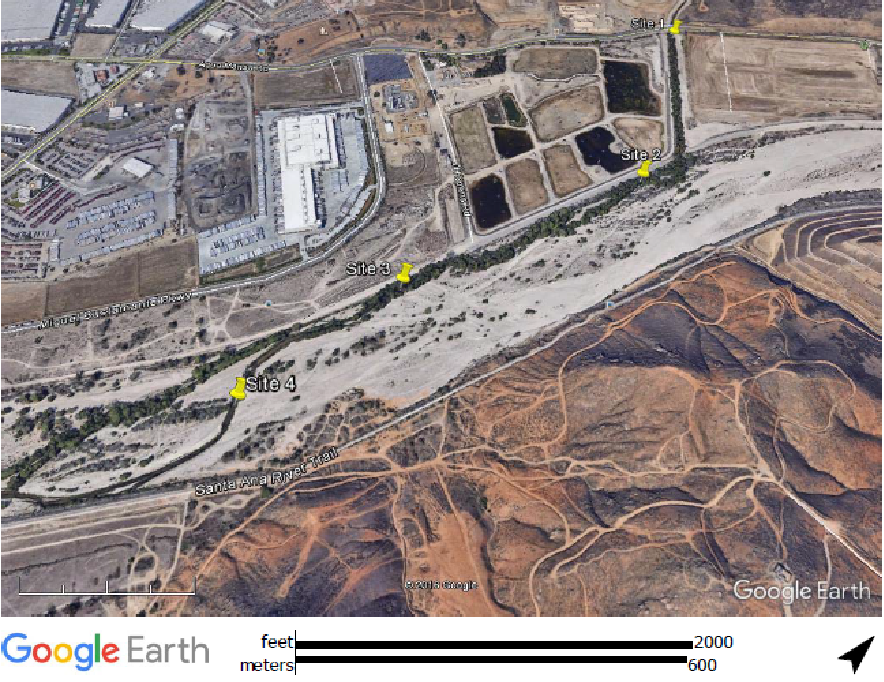
\includegraphics[width=1.00\textwidth]{Figures/SiteMap}
\caption{Sampling location maps}
\label{SAR_Image}
\end{figure}

The specific sites for our project included of one upstream location (Site 1) and one downstream location (Site 4), located approximately one kilometer apart (Table \ref{tab:sitedescription}). Site 1 was characterized by the presence of large debris, e.g., rocks and branches. In contrast, the river at Site 4 was a plunge pool whose surface was relatively smooth. Site 2 was located in the Santa Ana River channel downstream of the Rialto channel. 

The clarity of the water made it possible to see that the stream benthos was composed of pebbles and small coarse sediments. The riparian characteristics of the river included native willows and sycamores and invasive  salt cedar (\emph{Tamarix}) and castor bean (\emph{Ricinus communis})  and some giant cane (\emph{Arundo donax}). 

\begin{table}
\caption{Description of sampling locations.}
\begin{tabular}{llll}\hline
Location & Latitude             & Longitude   & Description \\ \hline\hline
Site 1  &  TBD  & TBD  & Rialto Channel \\
Site 2  & 34\textdegree 2'29"N          & 117\textdegree 21'15"W   & Above RIX Influx \\
Site 3  & 34\textdegree 2'21"N          & 117\textdegree 21'20"W   & Below RIX Influx\\
Site 4  & 34\textdegree 2'5"N           & 117\textdegree 21"17"W   & Pool, approximately 40-50 cm in depth\\ \hline
\end{tabular}
\label{tab:sitedescription}
\end{table}


\subsection{Habitat Evaluation}

The collection of data on the algae abundance, sediment type, and vegetation canopy cover of the Santa Ana River was done along the section of the river described in the site description section on September 20th, 2016, from 1pm to 3:30pm. We evaluated 9 parameters from Sites 2-4, for a total of 27 measurements. At each site, beginning at Site 4, the following procedures were followed: 

\begin{enumerate}
\item A spot was chosen along the right bank. Each of the parameters were then measured.
\item For estimating algae abundance, we placed the 30  x 30 cm quadrat above the river bed and estimated the \% that was covered by algae to the nearest 10 \%.

\item The sediment type of the site was characterized as either fine or coarse based on the grain size of the 30x30cm section of stream bed covered by the quadrat as either fine or coarse. Coarse substrate was classified as anything larger than pebbles or sand, that is, larger than 6.5cm. If more than half of the area covered by the quadrat was coarse substrate, or fine substrate, the area was characterized as such respectively.

\item Canopy cover was measured from the same position as the algae by holding spherical canopy densiometer above water at elbow's length. Based on how many of the 15 intersections on the densiometer reflected overhead canopy, cover was then quantified on a 0-15 scale, 0 being the no canopy cover and 15 being full cover.

\item To measure temperature, we submerged the analog thermometer underwater and recorded the temperature in \textdegree C.

\item Qualitative aspects of the river, such as presence of a pool or of logs, were also noted at each measurement spot.

\item Each measurement was then also taken at the middle of the river and the left bank of the cross-section. 

\item Steps above were repeated at two cross-sections between 0 and 10 meters downstream both chosen using a random number generator for a total of 3 cross-sections along a possible total length of 20 meters, and 3 measurements at each cross-section, for a total of 9 measurements per site. 
\end{enumerate}

At each of the corresponding water sample collection sites, water velocity was also measured using a SonTek FlowTracker Handheld Advanced probe, which emits sonar waves at a certain depth in the water column, and based on the feedback (20 pings) gives a velocity reading. Ideally, multiple readings would be taken at each site, after the probe is placed on a flat section of the riverbed where water appears to be flowing net in the same direction. 

\subsection{Videography}

We acquired all the necessary equipment for an underwater filming project, keeping in mind the length of time we wanted to keep our cameras underwater. We chose the GoPro Hero 4 Silver because of its battery life and recording time. We also considered safety and theft prevention for the cameras, and for this reason decided to mount the cameras in cube-shaped cinderblock structures with one open side that we constructed ourselves. In the lab, we set up all the equipment, built the cinderblock structures, and prepared everything for the field. Once in the field, we selected appropriate data sites (sites 2 and 4), set up our cameras, and set them to record at morning and afternoon times throughout the day. After the data collection period, we collected the equipment from the river and did a fish count analysis of all the footage back in the lab. Initially, we tried counting the fish by placing an arbitrary line in the footage and only counting in that area. We counted during an interval of ten seconds As can be seen in Figure \ref{fig:wherefish}, fish were very hard to see in the footage. We later did a recount and counted all the visible fish in the video frame every minute for one hour of footage each in the morning and afternoon. More detailed information on these processes can be found in the appendix.

\begin{figure}
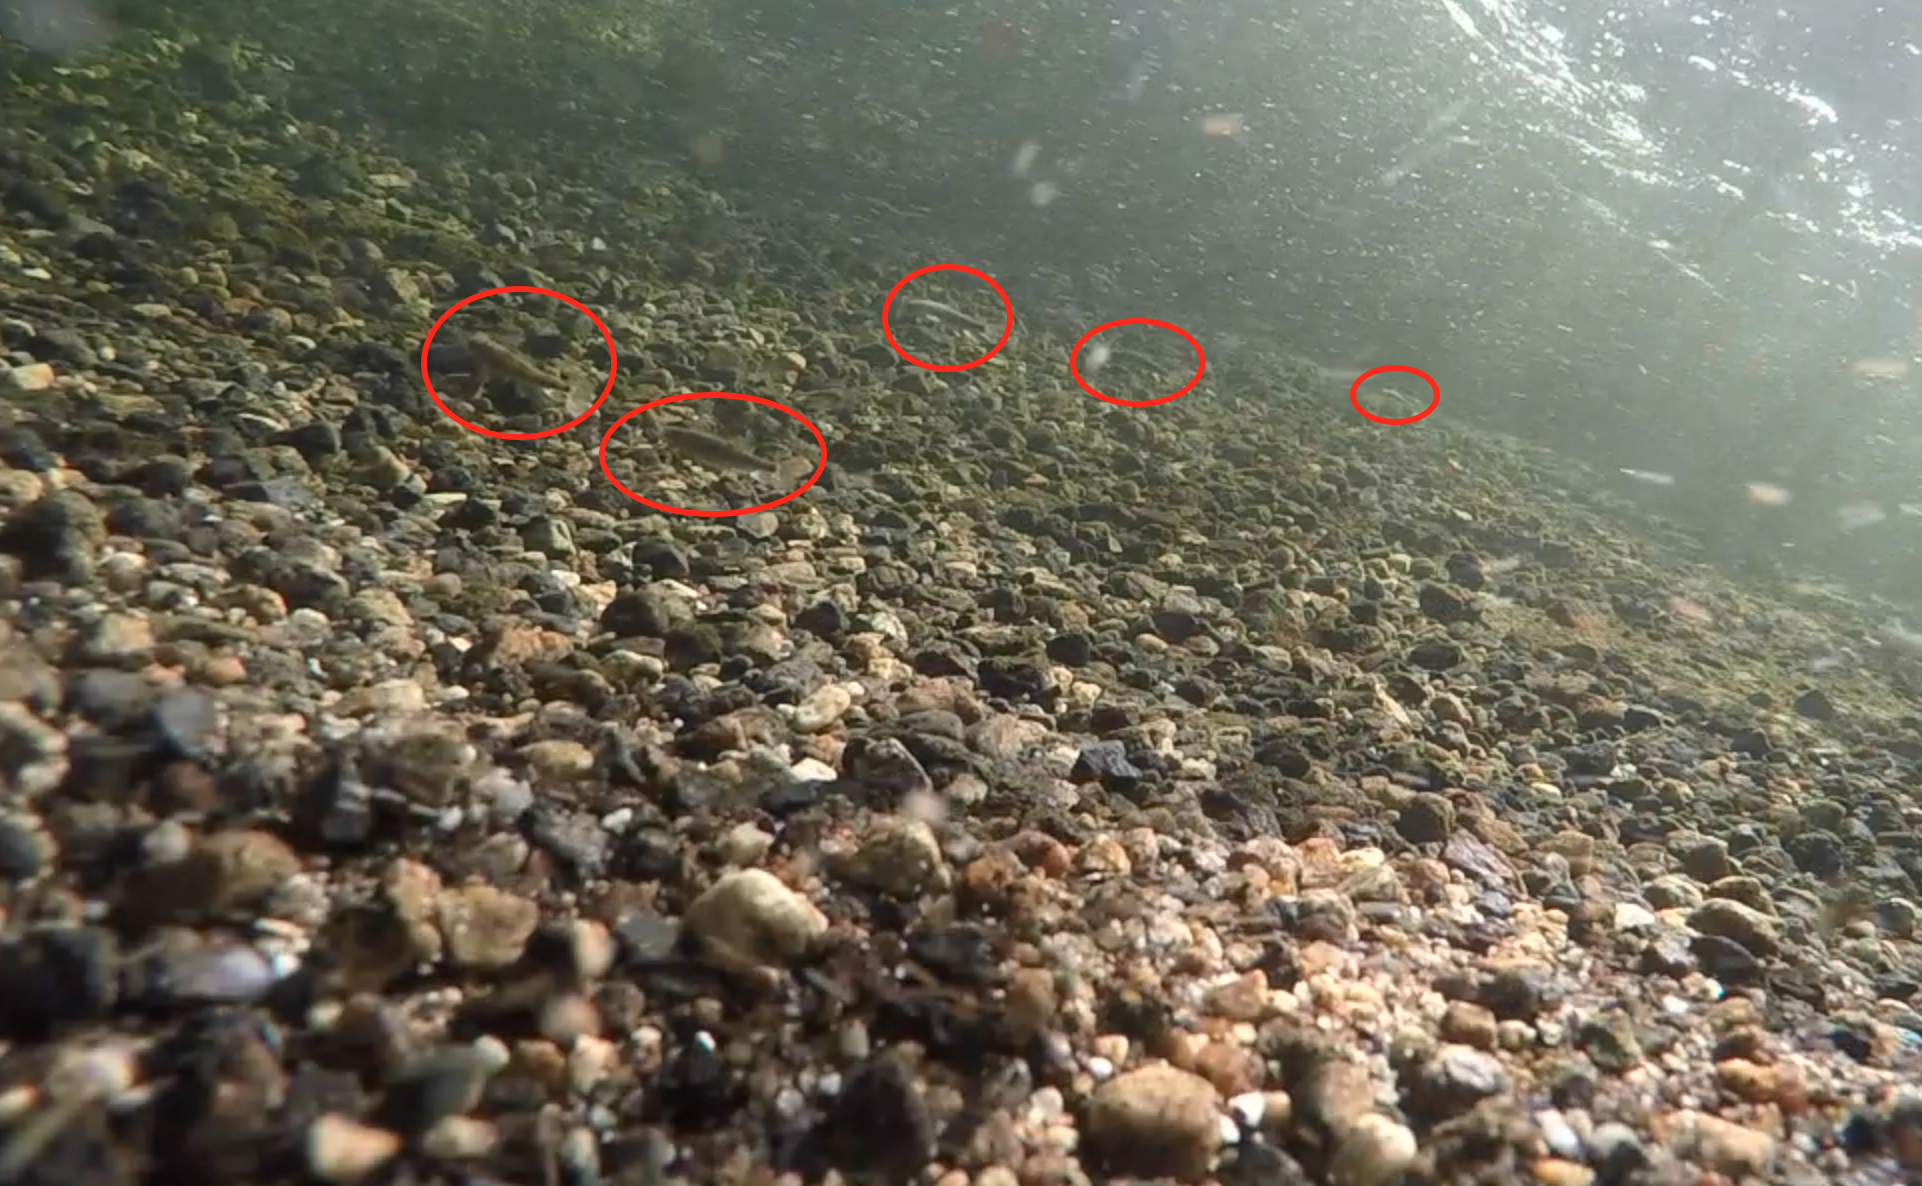
\includegraphics[scale=.4]{Videography_figures/wherefish}
\caption{The Santa Ana suckers were difficult to see in the underwater footage. Here, a few fish have been circled in the frame to showcase this. Because the fish were only clearly visbile when they were moving, it was necessary to count during a 10 second interval of footage.}
\label{fig:wherefish}
\end{figure}

\subsection{Temperature Loggers}

Temperature collection occurred from September 25th til October 1st for Site 2, and September 25th til October 4th for sites 1, 3, and 4, at 15 minute intervals. After collecting the field data, we calibrated each logger using an ice bath, and adjusted final temperatures based on differences in the ice bath.

\subsection{BOD Methods}

Approximately 1L of source river water was collected at each of two sites, one upstream location (Site 2) upstream of the RIX facilty and down stream of the confluence of the RIX facility and Rialto Channel (Site 4). BOD5 was analyzed using \citet{rice2012standard}. 

\subsection{Statistical Methods}

Using the R programming environment \citep{CRAN}, we use linear regression and ANOVA to analyze stream habitat variables. We also tested habitat value with fish count data comparing morning to afternoon counts. However, we acknowledge the fish count data are spatially and temporally autocorrelated, thus, our conclusions we make are serverely constrained based on the sampling methods.

\section{Results}



\subsection{Hydrology, Geomorphology, Canopy and Algae}

The average recorded water flow velocity was lower at Site 2, 0.27 ft/sec than Site 4, 1.09 ft/sec, where the difference was caused by a steeper channel gradient and a narrower channel width. 

The percent cover of the invasive algae may be influence by the stream substrate size (Figure \ref{fig:algae}, Panel A, p = 0.06). We found no relationship between the percent cover of the invasive algae species on the canopy cover (Figure \ref{fig:algae} Panel B, p = 0.334).

\begin{figure}[!ht]
\begin{knitrout}
\definecolor{shadecolor}{rgb}{0.969, 0.969, 0.969}\color{fgcolor}
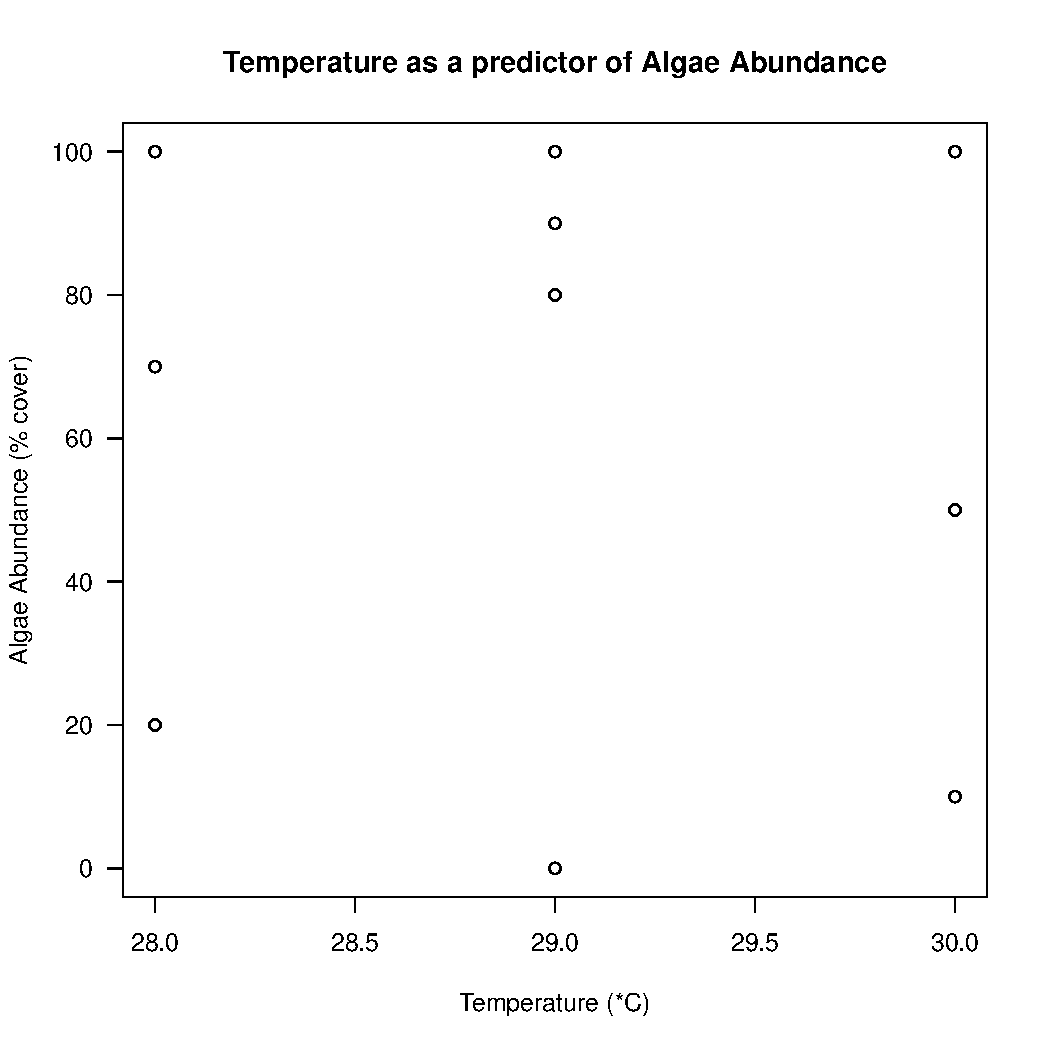
\includegraphics[width=5in,height=2.5in]{figure/unnamed-chunk-2-1} 

\end{knitrout}
\caption{Algae abundance as a function of the bed composition (Panel A), where course sediments = 1 and fine sediments = 0 and canopy cover (Panel B).}
\label{fig:algae}
\end{figure}

As an alternative method of analysis, we also analyzed to what extent site alone could predict algae abundance (Figure \ref{fig:algaesite}): site as a predictor was significant (p = 0.008).

\begin{figure}[!ht]
\begin{knitrout}
\definecolor{shadecolor}{rgb}{0.969, 0.969, 0.969}\color{fgcolor}
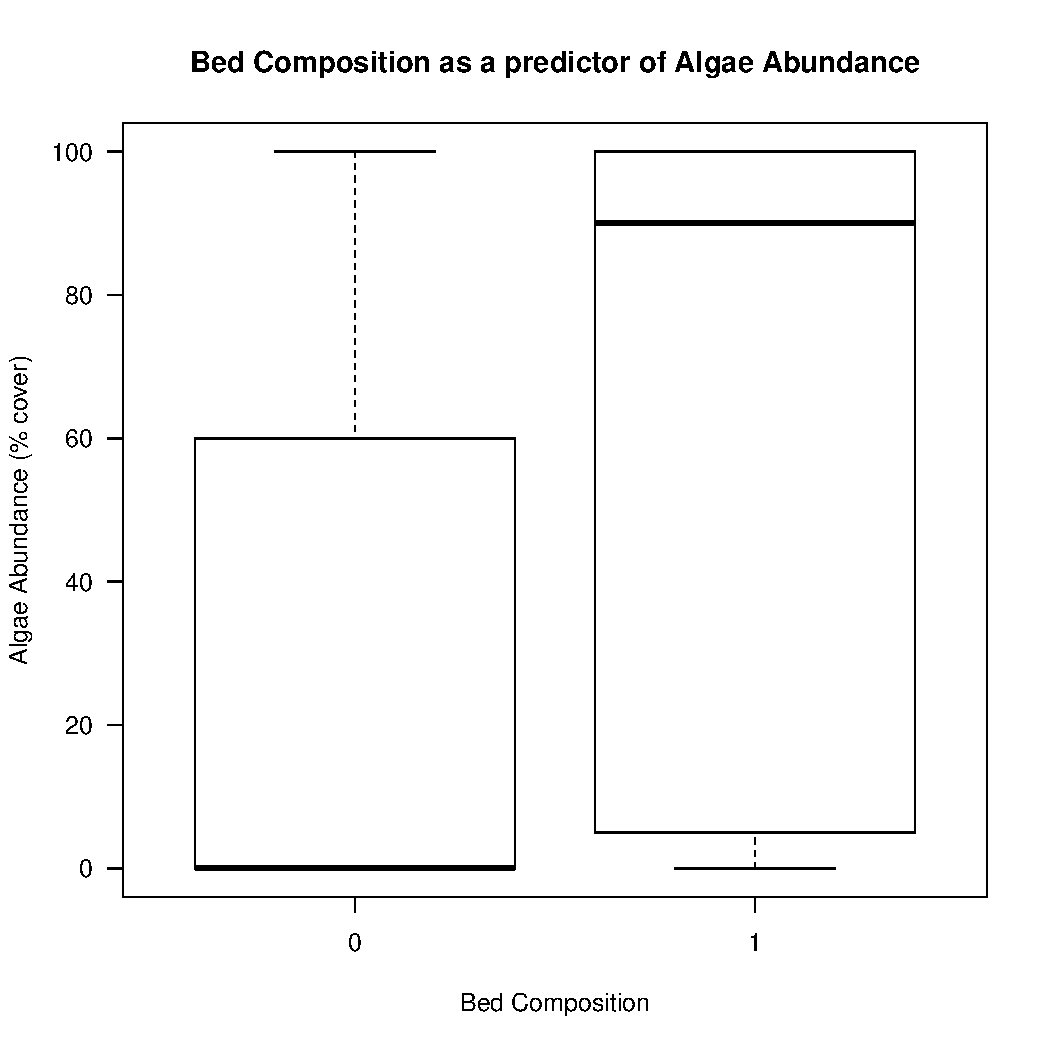
\includegraphics[width=\maxwidth]{figure/unnamed-chunk-3-1} 

\end{knitrout}
\caption{Algae abundance as a function of site.}
\label{fig:algaesite}
\end{figure}

\subsection{Water Quality Parameters}

Temperature fluctuated between a minimum of 25.1 \textdegree~C and a maximum of 31.4 \textdegree~C Celsius. The plunge pool, Site 4, had a mode of 27.5 \textdegree~C, which proved true for each locations, having the most repetitive temperature between 27 and 28 \textdegree~C. Site 4, however, had the least temperature range, only varying between 27 and 28.5 \textdegree~C, while other sites tended to have a bigger variation, with Site 1 varying up to 5.4 \textdegree~C. (Figures \ref{fig:Temp} and \ref{fig:boxplotTemp}).

The temperature patterns between the sites varied on a diel basis, where Site 2 consistently recorded the lowest temperatures in the early mornings, while Site 1 displayed the highest temperature in the late afternoon (Figure \ref{fig:Temp}). Although the end of the time series is lost for Site 2, the Site 1 is sometimes recording temperatures between Site 2 and Site 4 or matches the lows of Site 2 and 3. 

\begin{figure}
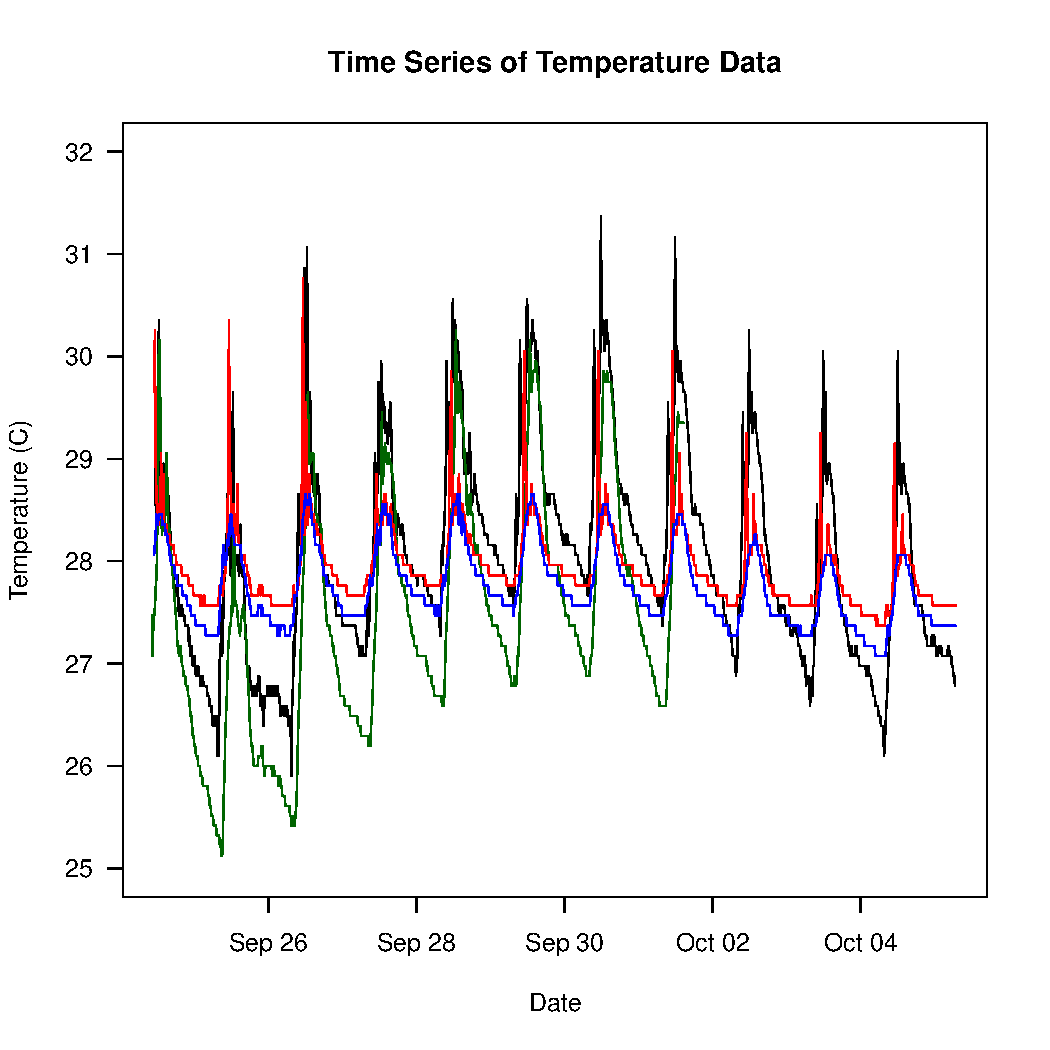
\includegraphics[width=0.90\textwidth]{Figures/Temp}
\caption{Temperature vs. time for all sites}
\label{fig:Temp}
\end{figure}

Site 4 had the narrowest range of temperatures and a median temperature that is between the other sites (Figure \ref{fig:boxplotTemp}). 

\begin{figure}
\begin{knitrout}
\definecolor{shadecolor}{rgb}{0.969, 0.969, 0.969}\color{fgcolor}
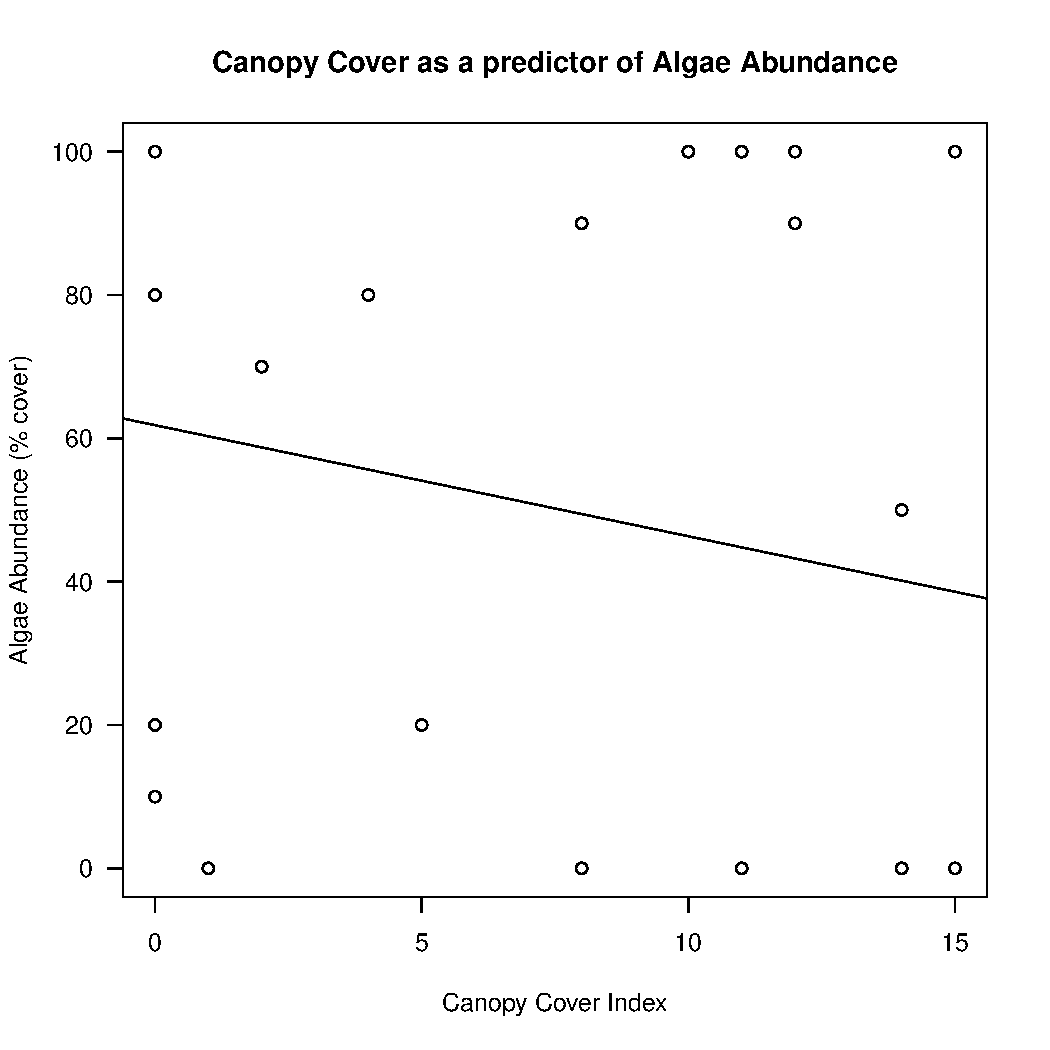
\includegraphics[width=\maxwidth]{figure/unnamed-chunk-4-1} 

\end{knitrout}
\caption{Temperature range for each site (\textdegree~C).}
\label{fig:boxplotTemp}
\end{figure}

We evaluated the relationship between algae abundance as a function of range of temperature (\textdegree~C) for each site (Figure \ref{fig:tempalgae}) and found no evidence that mid-day temperatures could predict algae abundance (p = 0.446), however, when we tested the temperature range we found a strong relationship to algae abundance (p $<$ 0.001, r$^2$ = 0.48), where higher temepature variation correlated with higher algae abundance, although this did not include Site 1, where the range was highest and no algae was sampled.

\begin{figure}[!ht]
\begin{knitrout}
\definecolor{shadecolor}{rgb}{0.969, 0.969, 0.969}\color{fgcolor}
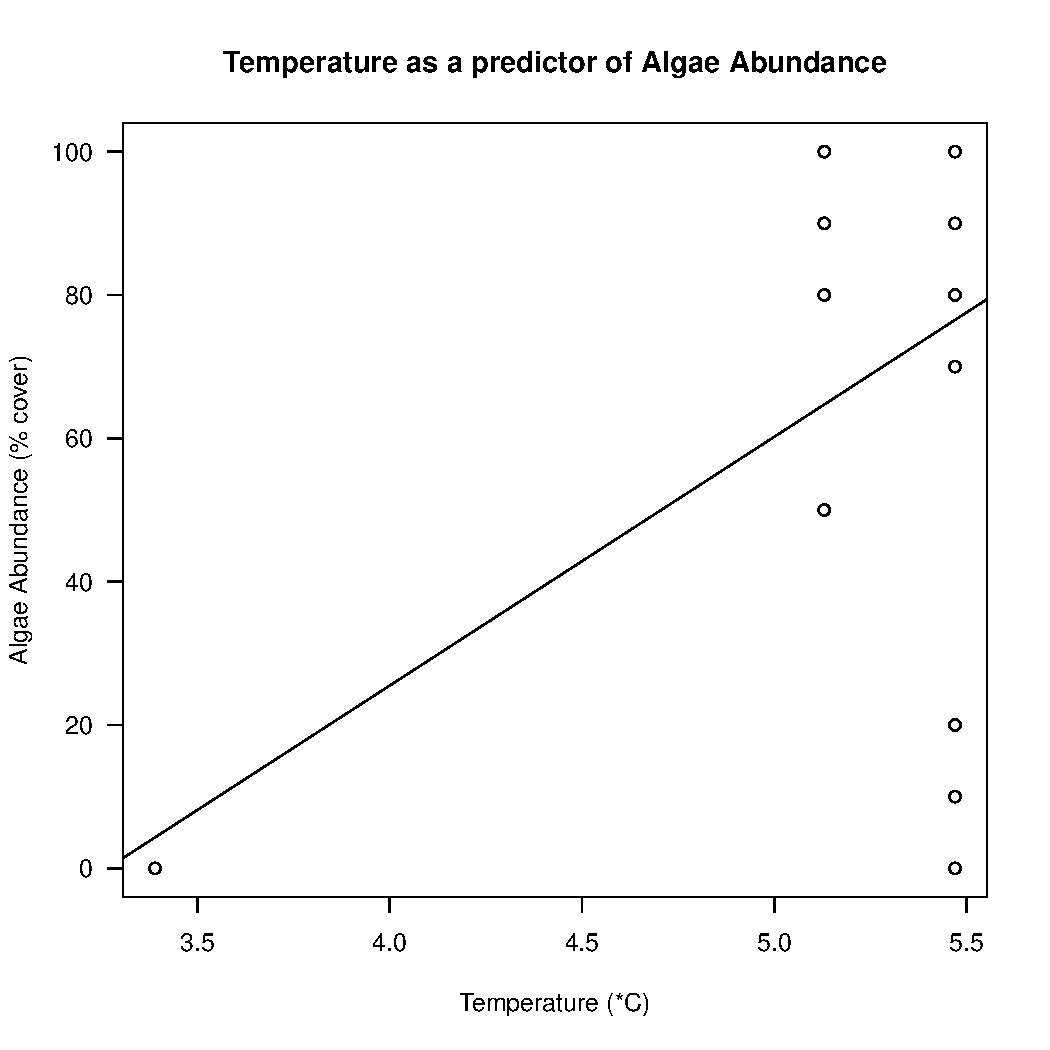
\includegraphics[width=\maxwidth]{figure/unnamed-chunk-5-1} 

\end{knitrout}
\caption{\emph{Cosmopogen aeruginosus} abundance as a function of temperature.}
\label{fig:tempalgae}
\end{figure}

Analysis of the data using quality control parameters indicated that two source water samples met minimum DO depletion standards. Site 4 had a higher BOD$_5$, 27.3 mg/L, and upstream site, Site 2, had a lower BOD$_5$ with 22.1 mg/L. 

\subsection{Fish Counts}

Counting the suckers relied on videography because still fish were well comoflauged and difficult to see (Figure \ref{fig:reallygoodcrop}). However, when use in conjunction video, fish could be counted because their swimming distinquished them from their surroundings.

\begin{figure}
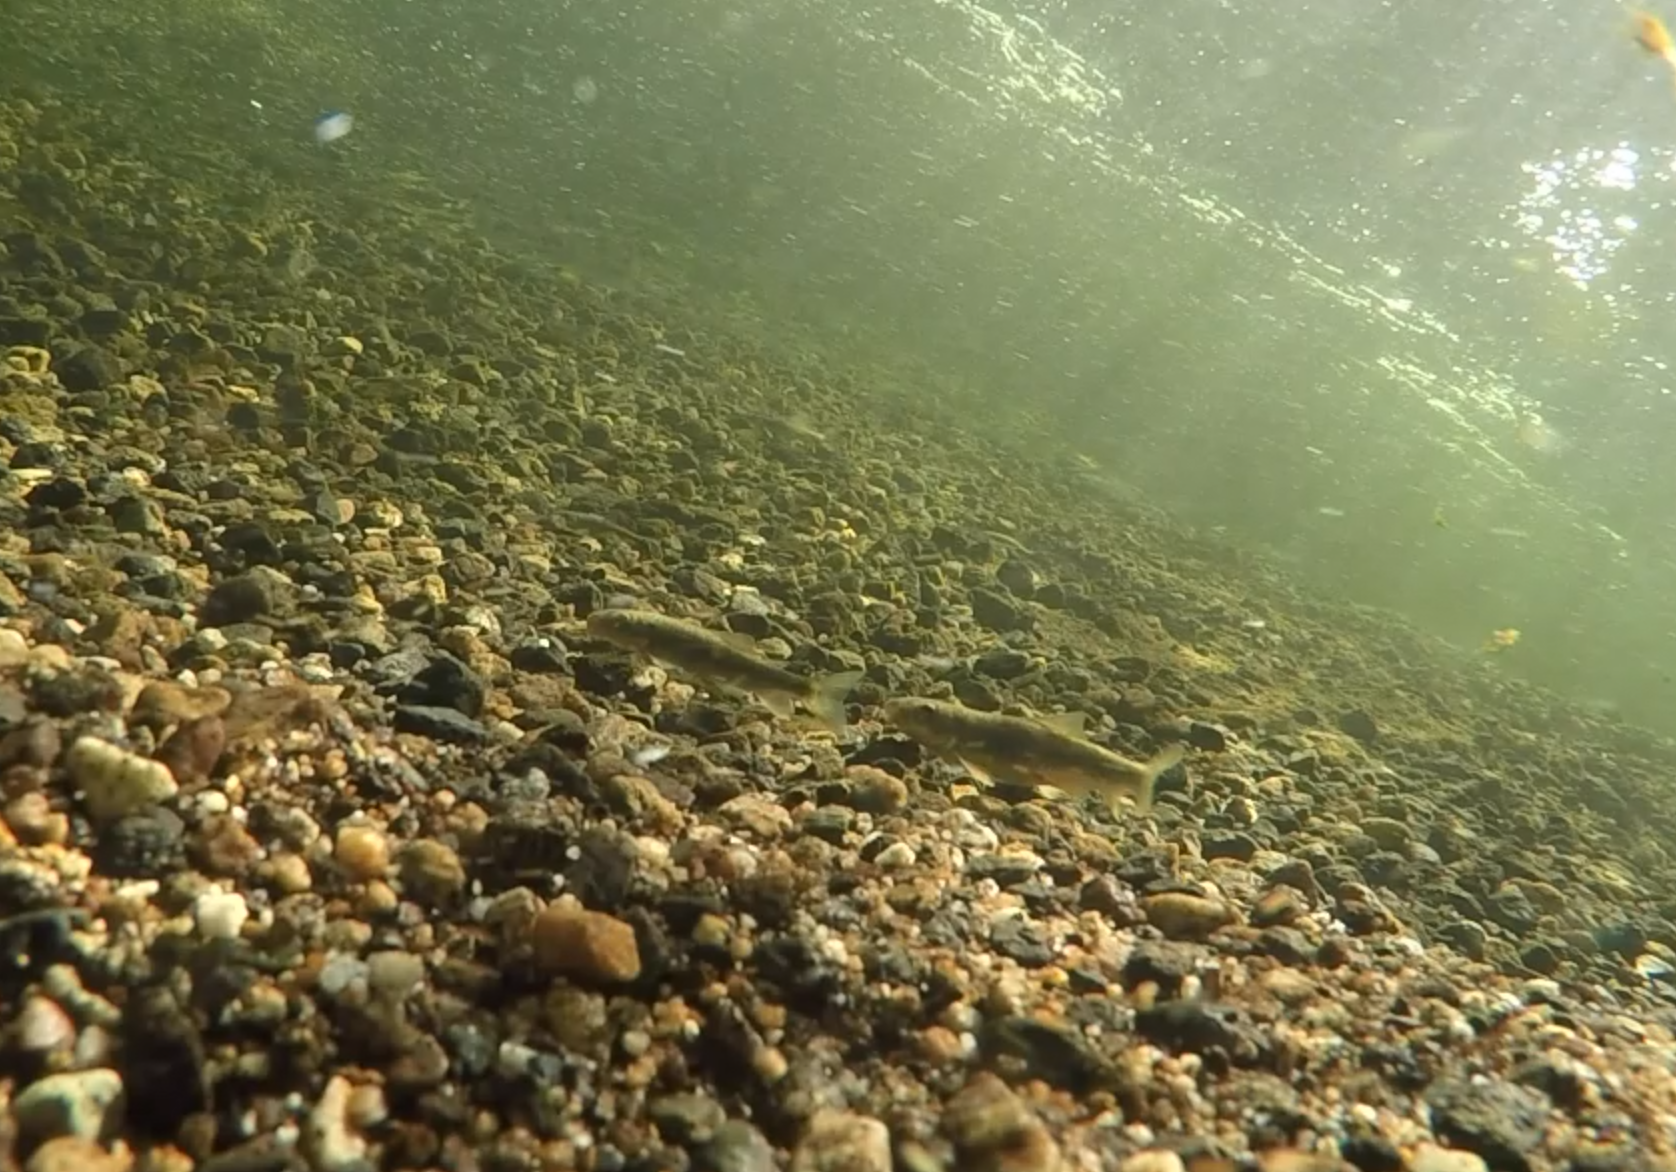
\includegraphics[scale=.4]{Videography_figures/reallygoodcrop}
\caption{A close up of two Santa Ana suckers from the footage we collected.}
\label{fig:reallygoodcrop}
\end{figure}



\begin{table}[!ht]
\caption{Videography Fish Count Summary Statistics at Site 4}
%\begin{tabular}{ |p{1.5cm}||p{1cm}|p{1cm}|{p2cm}|{p2cm}|{p2cm}|{p2cm}|{p2cm}|  }
\begin{tabular}{cccccccc}
 \hline
 \multicolumn{8}{c}{Summary Statistics} \\
 \hline
 Section & Min & Max & Mean & Median & 1st Quartile & 3rd Quartile & K\\
 \hline
 Morning & 7 & 29 & 20.13 & 22  & 16.75 & 25 & -0.6\\
 Afternoon & 14 & 49 & 32.25 & 31 & 24.75 &  42 & -1.3\\
 \hline
\end{tabular}
\label{tab:fishcounts}
\end{table}

At the upstream location (Site 2), no suckers were observed in the morning while one sucker occasionally swim out from behind a rock. At the downstream location (Site 4), we observed numerous fish for throughout the recorded video times (Table \ref{tab:fishcounts}). We counted an average of 20.1 suckers in the morning with a standard deviation of 6.0 fish.  In the afternoon, we counted an average of 32.2 with a standard deviation of 9.9, meaning both the average and the variance were higher in the afternoon (Figure \ref{fig:fishsection}, p $<<$ 0,001).  The river was 27.8\textdegree C in the morning and increased to 28.4\textdegree C in the afternoon. 

\begin{figure}[!ht]
\begin{knitrout}
\definecolor{shadecolor}{rgb}{0.969, 0.969, 0.969}\color{fgcolor}
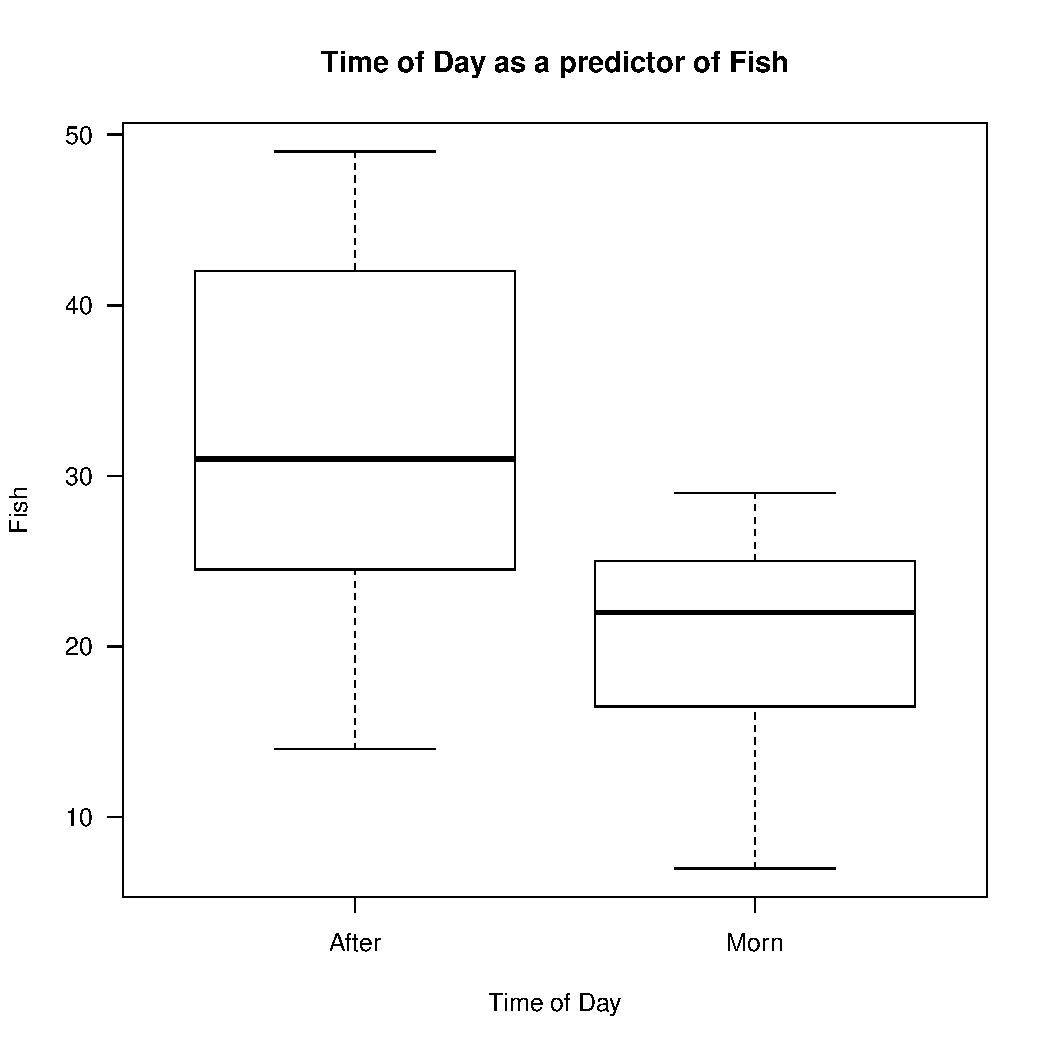
\includegraphics[width=\maxwidth]{figure/unnamed-chunk-7-1} 

\end{knitrout}
\caption{Fish counts as a function of time of day at Site 4}
\label{fig:fishsection}
\end{figure}

\section{Discussion}

\subsection{Habitat Quality and Fish Activity}

\subsubsection{Hydrology and Geomorphology and Algae}

Algae cover was a function of several predictors that could not be disentangled. For example, algae abundance between the 3 sites examined in our study, but that might have been a result several factors. Some measurements showed up to 100\% algae cover, while others exhibited none. This variation suggests the possibility that algae may be controlled by specific variables. We tested whether water temperature, water temperature variation, canopy cover, or stream bed composition could explain these variations. Of these possible causal factors, we found the strongest evidence for higher water temperature variation exerting a positive effect of algae abundance. The relationship between algae cover and streambed sediment composition of the stream bed was not statistically significant at the 95 \% level, but did tentatively suggest that algae may prefer coarse sediment. \emph{Cosmopogen aeruginosus} in the Santa Ana River has a highly unequal distribution, that appears to be controlled in part by water temperature variation, with a possible small contribution of streambed sediment composition. Our exploratory study is one of the first to examine what variables may control \emph{Cosmopogen aeruginosus}'s distribution in the Santa Ana River. 

This indicates that there is probably some relationship between algae cover and sediment composition of the stream bed, and this should be examined in future. In general, alage seem to perhaps prefer coarser sediment. 

\subsubsection{Temperature and Invasive Algae}

The temperature data include spikes on a daily basis, which were especially significant Sites 1 and 2. For example, Site 1 fluctuated up to 5.4 \textdegree~C a day. Our original hypothesis when we saw this was to assume water spikes were occurring from the Rialto Channel and as they travelled down river, becoming less extreme. In additioin, we did not find a temperature spikes traveling downstream. In fact, the spikes further downstream were actually occurring before the spikes upstream. We are unsure why there were such fluctuations in the river, because it did not appear that spikes were travelling downstream, based on the times that high and low temperatures occurred at different points in the river. In addition, all the temperatures that were measured were well above 22 \textdegree~C, which is the optimal temperature for the fish \citep{usfishandwildlifeservice14}. The lowest temperature found was 25.1 \textdegree~C. 

In similar studies, variations in stream temperature due to runoff were logged every 5 minutes, were found to have a negative impact on trout and the aquatic system in general \citep{jones2007effect}. The temperature disproportinately affects fish eggs and young fish, as the greate surface-area to volume ratio deters the eggs/young from being able to regulate body temperature \citep{Nelson09} . In small Piedmont streams, it is estimated that 50-70 percent of fish will be stressed given future climate and urbanization predictors, with temperature causing significant changes in both juvenile and adult growth. Thermal tolerance from native fish proved to have a greater range, while native fish, compounded by other factors such as food availability and spawning substrate, struggled. This study modeled climate change affects on the environment for the next ten years, seeing that climate change will not only effect water temperature but also precipitation, which will further stress out fish populations \citep{Nelson09}.

\subsubsection{Fish Behavior and Counts}

In terms of fish population, using the data from the Fish and Wildlife Service and our video data, no suckers were found at Site 1, only one fish counted in the afternoon at Site 2 at various points, no fish were found by the FWS at Site 3, but many fish were observed in the plunge pool at Site 4. Also, from previous results, we knew that most Santa Ana suckers live in the plunge pool and prefer it there. This could be because of reasons other than temperature, but we did notice that there were less extreme spikes in Site 4. Our videos of Site 2 contained very few fish. 

This could be because the temperature further upstream was too hot for the suckers to live in; the temperature data found that at that location the water was between 30.25\textdegree~C in the afternoon and 25.12\textdegree~C in the morning. This is a range of 5.13\textdegree~C, which is a much larger range than the range found at Site 4, where more suckers were found. In general, the fish were more abundant downstream, where the least extreme temperature spikes were occurring. From what we observed, the extreme temperature spikes at sites 1 and 2, and the medium spike at Site 3, could have caused the fish to prefer to stay at Site 4, where they are most abundant. This disproves our null hypothesis that the fish would be randomly spread throughout the channel and that temperature would remain fairly constant throughout the river, which suggests there could be a correlation between what is happening temperature wise and with the location of the suckers.

Also, the hottest temperatures that occurred at Site 2 were almost at mortality rate for suckers, and were 1.59\textdegree~C higher than any temperatures found in Site 4. It is possible that the fish prefer Site 4 for other reasons than temperature, but correlations between temperature and sucker abundance should be further explored.

Significantly more suckers in the afternoon than there were in the morning (p < 0.001).  Perhaps, suckers do move downstream throughout the day to get to cooler temperatures.  On the afternoon we tested, the plunge pool (downstream) was 28.5\textdegree~C, whereas the river at our upstream location, closer to the concrete, was 29.4\textdegree~C. Throughout our longer term temperature testing, we noticed there was significantly more variation in temperature the further upstream we tested. These large temperature spikes and variability could have prevented fish from successfully habitating the upstream sites.

There were also pretty extreme spikes, but not occurring at times that suggested spikes were travelling downstream, originating from the Veolia water plant. Initially, Veolia agreed to send over their data on both the influx and outflux water temperatures, to allow us to see what was happening to water temperature from the plant. However, after a week of following up, we have not been able to get the data, as the CPO has hesitated to release it and says it will take up to a month to compile it. Without this data, it is hard to explain these randomly occurring spikes at different points in the river. This part of the data could have also been affected by canopy cover or stratification. 

It is difficult to determine if the temperature spikes were what caused the fish to choose to reside primarily in Site 4, because there are a myriad of other variables. Other variables that could have affected where the fish chose to live include algae/food source, canopy cover, depth, or sediment type/size. What we do know is that the further upstream locations not only had a wide range of temperatures, but also experienced hotter temperatures than Site 4, which was where the fish live. From our background research, we know that the US Fish and Wildlife Service found that Santa Ana suckers prefer water that is around 22 \textdegree~C. None of our sites had water this cold, but Site 4 had the least variability and averaged around 28 \textdegree~C. According to a brief overview from Larry Brown of the US Geological Survey, no fish were detected at Site 1, while a few European chubs were sampled at sites 2 and 3. At Site 4 they estimated large numbers of fish but did not conduct a formal survey of this site. However, our video data showed a much larger population in the plunge pool. These population estimates were the results of random surveying, and could be limited in their applicability because of variation in site location and scope. For example, Larry Brown measured sucker populations in the Rialto drainage but not in the pool below it, which is where we placed our data logger \citep{perscomBrown}. Therefore, it is difficult to tell to what extent the US Geological Survey's data works with our data. 

\subsection{BOD$_5$}
Future study of dissolved oxygen levels and water velocity in the Santa Ana River should test for any correlations with the recent Fish and Wildlife Service electroshock population data. Though we did not have access to this data, we had access to a rough estimate of the sucker population from video-counting (mentioned above). Over the course of four hours, about 12 fish were counted at Site 2 and 671 fish at Site 4. So, many more fish were spotted where the river velocity was higher and where the BOD$_5$ levels were higher. Since BOD can be less than 2 mg/L in clear water and reach hundreds of mg/L in organic waste water, a difference of about 5 mg/L between Site 2 and Site 4 is very small. It is unlikely a threshold was reached between 22.1 and 27.3 mg/L that changed the habitat quality of Site 2 for the sucker. \citet{chattopadhyay1988study} note in their study of the effect of BOD on nutrient concentration, primary productivity, and dissolved oxygen variations that 10-20 ppm is the optimum range for fish incorporated into wastewater systems. Finally, in a study done by \citet{mallya2007effects} on the effects of dissolved oxygen on Atlantic halibut growth in aquaculture, the growth rate was found to be higher when the oxygen level was between 80\% and 120\%, and the feed conversion ratio was lower at 120\% saturation. The difference in velocity is more significant and also supports the referenced existing literature that says water flow velocity is one of the primary determinants of sucker population \citep{evans2005draft, moyle2002inland, baskerville2012recovery}. We recommend future research on the Santa Ana sucker population focus on water velocity.

\subsection{Research Limitations}

Research efforts were limited a few sites and and a few weeks of field work. In particular, our research was unable to disentangle the relationship \emph{Cosmopogen aeruginosus}'s co-occurrence with sucker and other physical stream measures, such as temperature and streambed substrate characteristics. For example, recent RIX facility shutdown reduced algal biomass and had not recovered by our sampling dates. 

We were unable to characterize fish movement with the 2 underwater cameras, where an increase might better capture the temperal changes in fish behavior. In addition, developing a systematic way to count fish/frame would require additional method development.  

Water temperature measurements fluctuated but not necessarily with the air temperature measurements, averaged, from that day. Compared with the historic averages, the week of our experiment was particularly hot; thus, we may have captured fish behavior unrepresentative of the season. Furthermore, our sampling methods did not evaluate temperature stratification, which may be an important consideration in evaluating fish behavior \citet{sadler1980effect, matthews1994cool}.

\section{Conclusion and Recommendations}

The Santa Ana sucker may be impacted by the presence of \emph{Cosmopogen aeruginosus} and it's extensive growth. However, the number of confounding factors influencing the stream habitat, including median temperature, temperature range, canopy, and substrate made it impossible to assess the direct role of algae on the sucker. 

We recommend that developing a flume where fish behavior can be monitored while controlling a range of other factors. For example, a feeding choice test may provide the critical information to evalaute the role of periphyton species composition on the Santa Ana sucker.

\section{Literature Cited}

\bibliography{report}

\newpage
\section{Appendix: Detailed Methods}

\subsection{Video Camera Set up}

To set up the cameras, we removed them from the packaging, inserted a microSD card into each, and charged them fully by connecting the included USB cables to a computer. The cameras needed to be fully charged before we were able to adjust the settings. Once the cameras were sufficiently charged, we set the filming settings to record in 720p x 30fps. We set the cameras aside and left them charging. 

Next, we charged all four of the waterproof Re-Fuel battery packs. As these were charging, we put together our cinder block mounting structures. We took our cinder block cubes and set them up on a clean, stable table. We connected the flat adhesive mounts that were included with the GoPros and connected a GoPro camera to each. Since the cinder blocks were open on two parallel sides, we were able to see right through the cinder block cube to the other side. One of us stood on one side with the GoPro and mount, and the other stood on the other side of the opening. One of us turned the GoPro on and put the camera with the mount inside the cinder block cube, using the view on the screen to find the best position for the mount inside of the cube, taking care to ensure we could clearly see the other person on the other side. We found an ideal place where the view was mostly unobstructed by the sides of the cube but the cameras were still far enough inside the cube that they wouldn't be too easily spotted by passersby. This spot was 5 cm from the edge of the cube. We traced the front and the back of the mount so we could glue it in the correct place. We repeated this procedure for the second cube and mount, and standardized the construction by placing the mount in the second cube 5 cm away from the edge of the cube. 

In order to securely glue the mount in place, we used Gorilla glue. To activate the Gorilla glue, we first had to moisten one of the surfaces with water. We moistened the mounts on the adhesive side. We did not remove the adhesive backing so we could reutilize the mounts in the future. Once the mount was damp, we put Gorilla glue on the cinder block inside the lines we had drawn around the mount. We then placed the mount on the Gorilla glue, taking care to align the edges of the mount with the lines we had drawn. Next, as per the Gorilla glue instructions, we found a heavy object that could provide significant pressure on the mount and that would fit inside the cube. We left this for three hours to harden.

Upon returning to the lab, we removed the heavy objects from the cube and checked the seal on the mount and cinder block to ensure the bond had successfully cemented. After this, we went to work on attaching the cinder block backs to close up one of the open sides on the cubes. We repeated much of the same process we used when attaching the mounts to the cubes, and followed the Gorilla Glue instructions carefully. First, one of us moistened the cinder block back while the other applied Gorilla Glue to the edge of the cube. Then, we carefully aligned the corners of the back with the cube. We repeated this with the second cube. Seeing that the cinderblock back was heavy enough on it's own, we did not place a heavy object on top of this structure and instead simply left it to dry and harden overnight.

Finally, we checked on the cameras and battery packs again to ensure they had charged. We left them plugged in overnight. We also packed away the Gorilla Glue, the multiple SD cards, paper towels, and extra mounts in a field kit so we could deal with any emergencies in the field.

We started our first recording session at 10 am.  We drove to the downstream site and found a spot under brush cover in a pool next to a fast moving section of the stream.  We first placed the cinderblock squarely on the riverbed and positioned it facing the fast moving water.  We then turned the camera on, pressed record, and placed it on the mount in the cinderblock.  We let it run for a few seconds, then took it out and watched the video to ensure it was recording at a good angle.  We then pressed record again and replaced it.  Before leaving, we marked the area with flags so we would be able to find it again.
Next, we walked approximately 20 minutes upstream to another covered pool next to a fast moving section, and repeated the camera placement procedures.  We marked with flags, and then left.

We returned at approximately 2 pm.  We took out the camera at the downstream site, replaced the memory card and the battery pack, hit record, and replaced the camera exactly as it was positioned previously.  We then walked upstream and did the same thing with the second camera.  After returning, we cleared the memory cards and plugged in the battery packs.
Our last recording session was at 8 am the next morning.  We replaced the memory cards and battery packs again and returned the cameras to their positions.  One of us returned the next day to collect the cameras.

\subsection{Temperature Loggers}
We obtained four HOBO Tidbit water temperature Data Loggers to set up at the Rialto Channel at Agua Mansa (Site 4), another at the point where the other discharge site meets the river (Site 2), another just above that site (Site 3), and a fourth in the pool where suckers have previously been observed (Site 1). Before going to the river, In order to start the data process, we put each logger into the coupler and pushed the level til the light was flashing. We then put them in the river by looping a garden stake through one, sticking it into the substrate, and securing it with rocks. We then put yellow marking tape on plants nearby and red flags along the bank to show where we left the main path. We repeated this for each site, making sure the loggers were secure and fairly hidden. After seven nights (for Site 3) and eleven nights (for the other sites), we returned to the river and collected the loggers. In the lab, using the software, we loaded our data and transferred it to RStudio.

\subsection{$BOD_5$ Methods}

Ideally within the same day of collection, water samples were analyzed for initial dissolved oxygen content and prepared for 5-day incubation.  
\begin{itemize}
  \item Three different dilutions were used for each of two sites, with source water volumes of 25, 50, and 100 mL. 
  \item A seed suspension was prepared using PolySeed Seed Innoculum, and 4 mL of the solution was added to each 300 mL sample bottle. This solution was also used to create four seed blanks with seed volumes 15, 20, 25, and 30 mL.
  \item Nitrification inhibitor was created by dissolving 2.0 g allylthiourea (ATU, C4H8N2S) in 1 L distilled water. 0.3 mL of the ATU solution was added to each source water sample, as well as to all seeded samples. 
  \item A glucose-glutamic acid (GGA) solution was prepared by dissolving 150 mg each of dry glucose and glutamic acid in 1 L of distilled water, and was added to each of the four seed blanks, as well as the six source water samples. Three GGA blanks were also created with 6 mL of GGA solution in incubation bottles. 
  \item Dilution water was created using 1 mL each phosphate buffer (8.5 g KH2PO4, 21.75 g K2HPO4, 33.4 g Na2HPO*7H2O, and 1.7 g NH4Cl dissolved in 1 L distilled water), Magnesium sulfate solution (4.5 g MgSO4*7H2O dissolved in 200 mL distilled water), Calcium chloride solution (5.5 g CaCl2 dissolved in 200 mL distilled water), and Ferric chloride solution (0.05 g FeCl3*6H2O dissolved in 200 mL distilled water), and added to the six source water samples, four GGA blanks, and three seeded blanks. Three dilution water blanks were also created using the same procedure diluted to 300 mL.
\end{itemize}
Initial DO readings were to be taken on all blanks and samples using a Thermo Scientific DO Probe with auto-spinning functionality. The bottles were then incubated in a dark area for 5 days, and DO readings were again taken.  

Note that *Temp\_x* entries were borrowed with permission from Sophie and Nicole's dataset. We also created a "Site\_New" field so that our naming conventions whould be consistant with other teams. We then used rstudio to generate the following descriptive statisitcs:  
linear regression of temperature range vs algae abundance
linear regression of canopy cover vs algae abundance
ANOVA of bed composition vs. algae abundance
ANOVA of site location vs. algae abundance
For each of these statistical comparisons, we tested whether we could reject the null hypothesis, and if yes, discuss the implications of those findings. Our results are summarized in the following section. 

\subsubsection*{Quality Control Checks}
Using the seed blanks, glucose-glutamic acid blanks, and dilution water blanks, quality control checks were performed prior to data collection. 
\begin{itemize}
  \item Minimum DO Depletion--Viable samples must have min. DO depletion of 2.0mg/L, and residual DO of at least 1.0mg/L.
  \item Glucose-Glutamic Acid Check--The resulting average BOD for the 3 GGA blanks (after correction for dilution and seeding) must be 198+/- 30.5mg/L.
  \item Dilution water check--DO uptake after incubation must not be more than 0.20mg/L and preferably not more than 0.10 (before seed corrections). 
  \subitem Dilution Water--If dilution water blank exceeds 0.20 mg/L, clearly identify samples in data.
  \item Seed control--Calculate Seed Control Factor (SCF) using 
  \begin{equation}
  [(D1-D2)*f], 
  \end{equation}
  where
  \subitem $D_1$= initial DO of seed control, mg/L
  \subitem $D_2$= final DO after indubation, mg/L,
  \subitem f= (vol. seed in diluted sample)/(vol. seed in seed control)
\end{itemize}

\subsubsection*{BOD5}
BOD5 was calculated for viable samples according to Standard Methods for the Examination of Water and Wastewater, using the equation 
BOD5,
\begin{equation}
mg/L= ((D_1-D_2)-(S)V_s)/P,
\end{equation}
where 
\subitem $D_1$= initial DO, mg/L
\subitem $D_2$= final DO after incubation, mg/L
\subitem S= oxygen uptake of seed, ∆DO/mL of seed suspension added per bottle
\subitem $V_s$= volume of seed in test bottle
\subitem P= decimal volumetric fraction of sample used.
The average of the resulting values for all viable samples was determined, and reported as our results. 


\end{document}
